\documentclass[aspectratio=169]{beamer}
\usepackage{babel}

\usepackage{array, colortbl, transparent, listings}
\usepackage[export]{adjustbox}
\usepackage[skins,theorems]{tcolorbox}
 
\setbeamercovered{transparent}

\title{Rust vs C++: Brief Introduction}
\author{Anatoly Weinstein}
\date{30th of April 2025}

\newcommand{\framebackground}[2]{
    \begin{tikzpicture}
        \transparent{#1}
        \node[inner sep=0] at (current page.center) {
            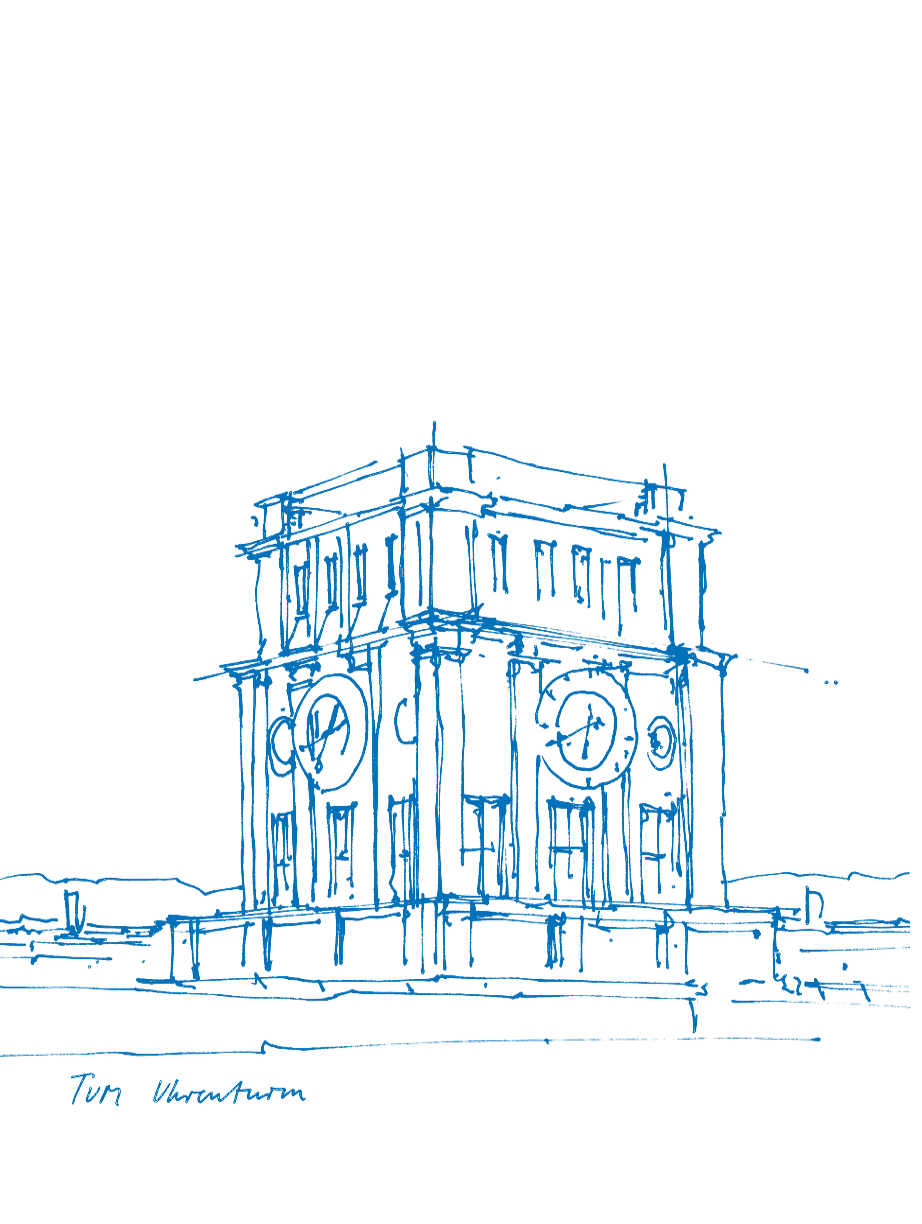
\includegraphics[height=\paperheight, right]{./media/tum-uhrenturm.png}
        };
        \transparent{1}
        \node[anchor=south, text width=\paperwidth, text height=1.5cm, draw=none, align=center] at (current page.south) {
            \insertpagenumber
        };
        \transparent{#2}
        \node[anchor=south, text width=\paperwidth, text height=1.5cm, draw=none, align=right] at (current page.south) {
            \small Anatoly W. \,\,
        };
    \end{tikzpicture}
}

\newcommand{\headerframe}{
    \usebackgroundtemplate{
        \framebackground{0.2}{1}
    }
}

\newcommand{\simpleframe}{
    \usebackgroundtemplate{
        \framebackground{0}{1}
    }
}

\newcommand{\blue}[1]{{\color{beamer@blendedblue} #1}}
\newcommand{\yellow}[1]{{\color[HTML]{AF8F10} #1}}
\newcommand{\gray}[1]{{\color[HTML]{8F8F8F} #1}}
\newcommand{\red}[1]{{\color[HTML]{FF5F5F} #1}}

\begin{document}

%
% Frame
%
\usebackgroundtemplate{\framebackground{0.2}{0}}
\begin{frame}
    \maketitle
\end{frame}

\simpleframe\begin{frame}{Commands and Tooling}
    \begin{tabular}{ m{0.45\textwidth} | m{0.45\textwidth} } 
        \textbf{Rust} & \textbf{C++} \\
        \hline
        \texttt{cargo build} & \texttt{make} \\
        \texttt{cargo run} & \texttt{make run} \\
        \texttt{cargo test} & \texttt{make test} \\
        \\
        \texttt{cargo fmt} & \texttt{clang-format} \\
        \texttt{cargo clippy} & \texttt{clang-tidy} \\
        \\
        \texttt{./target/debug/pse-mol} & \texttt{./pse-mol.a} \\
    \end{tabular}
\end{frame}

\simpleframe\begin{frame}{Ferris will answer questions}
    \centering
    % image from:
    % https://en.wikipedia.org/wiki/List_of_computing_mascots
    
\includegraphics{media/ferris.png}
\end{frame}

\end{document}
